\section{Experiment and Result}
The aforementioned merged algorithm will be implemented in python to be tested. In this paper, the implementation will use PyTorch \cite{NEURIPS2019_9015} as library to build deep learning models and to get dataset. The experiment will be done in two scenarios, to see how the algorithms performs under different conditions. For each experiments, the quantization function that will be used is the mapping from float64 data type to float16 data type. This quantization function fulfills \autoref{quantdef} and is simple to implement in PyTorch.

For all experiments, the accuracy will be tracked to measure how each algorithm affects model training. The experiments will also record the communication rounds needed and the data size used for communications. Then, each algorithm will be compared in each aspect.

\subsection{Fashion-MNIST}
The first experiment scenario is to train a simple model on Fashion-MNIST dataset \cite{xiao2017fashion}. This is a simple computer vision dataset aimed to replace MNIST dataset. For the model, a simple model with 2 convolution-maxpooling layer and a fully-connected layer will be used. Architecture of the model can be seen in \autoref{simplemodel1}.
\begin{figure}[htbp]
  \centering
  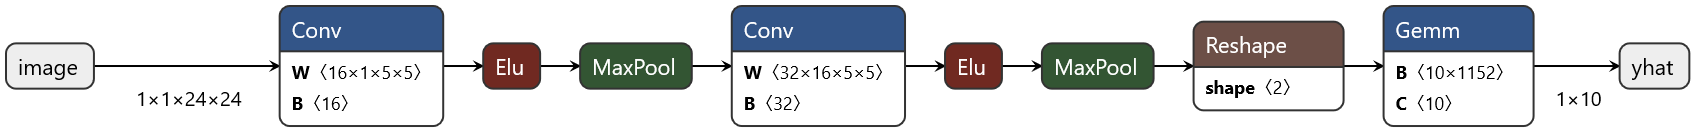
\includegraphics[width=0.8\columnwidth]{resources/fashion_mnist.onnx.png}
  \caption{\label{simplemodel1}A simple model for classifying Fashion-MNIST}
\end{figure}

The choice of hyperparameter for this scenario can be seen in \autoref{hyperparamfashion}

\begin{table}[htbp]
  \caption{\label{hyperparamfashion}Hyperparameter choice for Fashion-MNIST classification}
  \centering
  \begin{tabular}{ | c | c | c | }
    \hline
    \textbf{Algorithm}                                       & \textbf{Hyperparameter} & \textbf{Value} \\
    \hline
    \multirow{5}{*}{CADA \cite{Chen2021CADA}}                & $\alpha$                & 0.00001        \\
                                                             & $\beta_1$               & 0.9            \\
                                                             & $\beta_2$               & 0.99           \\
                                                             & $D$                     & 50             \\
                                                             & $d_{max}$               & 10             \\
                                                             & $c$                     & 400            \\
    \hline
    \multirow{3}{*}{Efficient-Adam \cite{Chen2022Efficient}} & $\alpha$                & 0.0001         \\
                                                             & $\beta_1$               & 0.9            \\
                                                             & $\beta_2$               & 0.999          \\
    \hline
    \multirow{5}{*}{Merged Algorithm}                        & $\alpha$                & 0.0001         \\
                                                             & $\beta_1$               & 0.9            \\
                                                             & $\beta_2$               & 0.99           \\
                                                             & $D$                     & 50             \\
                                                             & $d_{max}$               & 10             \\
                                                             & $c$                     & 400            \\
    \hline
  \end{tabular}
\end{table}

Results of experiment in this scenario are shown in \autoref{fashionacc1}, \autoref{fashionbits1}, and \autoref{fashioncomms1}. From these graphs, it could be seen that the resulting accuracy for each algorithm varies, with Efficient-Adam in the lead at around 86\%. There is no reduction of communication in all algorithms, but Efficient-Adam manages to reduce needed communication data size to just around 0.3 times that of CADA. The merged algorithm showed a reduction in communication data size, but still needed more communication data size than Efficient-Adam.

\begin{figure}[htbp]
  \centering
  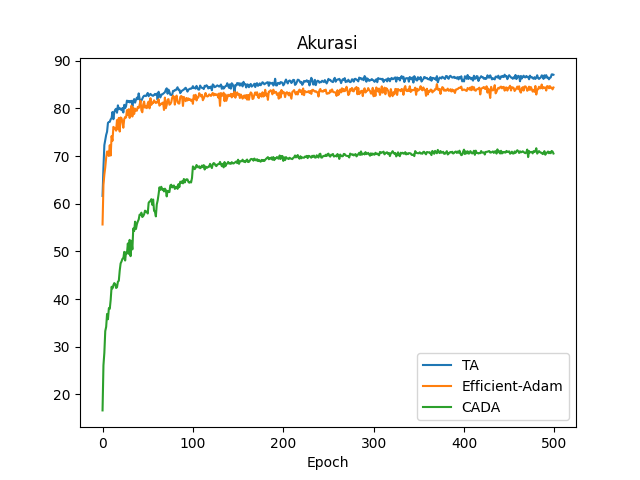
\includegraphics[width=0.8\columnwidth]{resources/fashion_acc.png}
  \caption{\label{fashionacc1}Accuracy for each algorithm in Fashion-MNIST scenario}
\end{figure}
\begin{figure}[htbp]
  \centering
  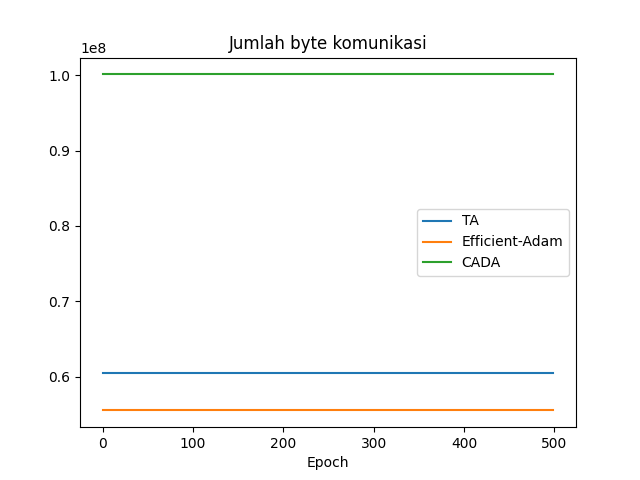
\includegraphics[width=0.8\columnwidth]{resources/fashion_bits.png}
  \caption{\label{fashionbits1}Communication data size used for each algorithm in Fashion-MNIST scenario}
\end{figure}
\begin{figure}[htbp]
  \centering
  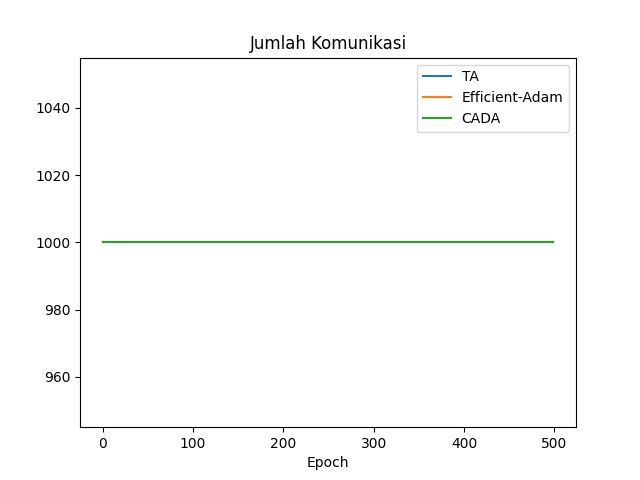
\includegraphics[width=0.8\columnwidth]{resources/fashion_comms.png}
  \caption{\label{fashioncomms1}Communication rounds for each algorithm in Fashion-MNIST scenario}
\end{figure}

\subsection{CIFAR-10}
The second experiment scenario is to train ResNet-18 \cite{he2015deep} on CIFAR-10 dataset \cite{krizhevsky2009cifar}. This paper chose ResNet-18 to represent a more complex deep learning model. The model has a total of around 0.27 million parameters in 20 layers. The building blocks of a ResNet model is a residual block, which can be seen in \autoref{resblock}.
\begin{figure}[htbp]
  \centering
  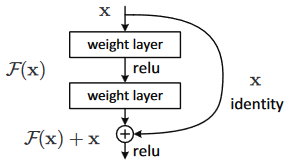
\includegraphics[width=0.8\columnwidth]{resources/resblock.png}
  \caption{\label{resblock}Residual block, from \cite{he2015deep}}
\end{figure}

The choice of hyperparameter for CIFAR-10 classification using ResNet-20 are show in \autoref{hyperparamcifar}
\begin{table}[htbp]
  \caption{Hyperparameter choice for CIFAR-10 classification}\label{hyperparamcifar}
  \centering
  \begin{tabular}{ | c | c | c | }
    \hline
    \textbf{Algorithm}                                        & \textbf{Hyperparameter} & \textbf{Value} \\
    \hline
    \multirow{5}{*}{CADA, \cite{Chen2021CADA}}                & $\alpha$                & 0.01           \\
                                                              & $\beta_1$               & 0.9            \\
                                                              & $\beta_2$               & 0.99           \\
                                                              & $D$                     & 50             \\
                                                              & $d_{max}$               & 2              \\
                                                              & $c$                     & 0.12           \\
    \hline
    \multirow{3}{*}{Efficient-Adam, \cite{Chen2022Efficient}} & $\alpha$                & 0.0005         \\
                                                              & $\beta_1$               & 0.9            \\
                                                              & $\beta_2$               & 0.999          \\
    \hline
    \multirow{5}{*}{Merged Algorithm}                         & $\alpha$                & 0.0005         \\
                                                              & $\beta_1$               & 0.9            \\
                                                              & $\beta_2$               & 0.999          \\
                                                              & $D$                     & 50             \\
                                                              & $d_{max}$               & 2              \\
                                                              & $c$                     & 0.12           \\
    \hline
  \end{tabular}
\end{table}

Results of experiment in this scenario are shown in \autoref{resnetacc1}, \autoref{resnetbits1}, and \autoref{resnetcomms1}. From the accuracy graph, it could be seen that all three algorithms performs similarly, with Efficient-Adam on the top again at around 86\%. In this experiment, CADA and merged algorithm both showed a reduction in communications. But, CADA only reduces communication in small scales, whereas the merged algorithm could reduce communications to under 875 around the 600\textsuperscript{th} epoch.

\begin{figure}[htbp]
  \centering
  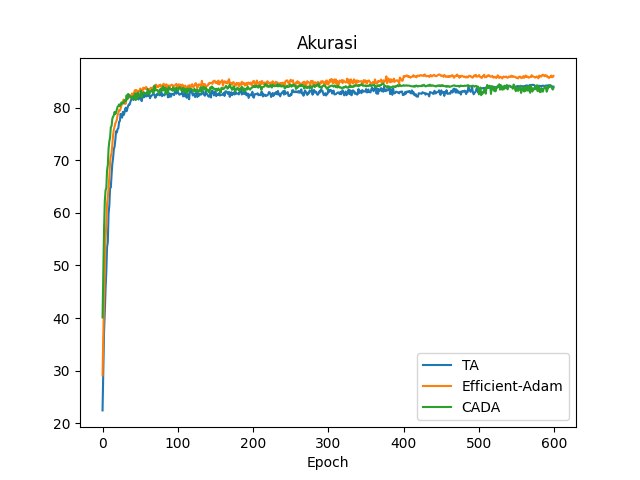
\includegraphics[width=0.8\columnwidth]{resources/resnet_acc.png}
  \caption{\label{resnetacc1}Accuracy for each algorithm in CIFAR-10 scenario}
\end{figure}
\begin{figure}[htbp]
  \centering
  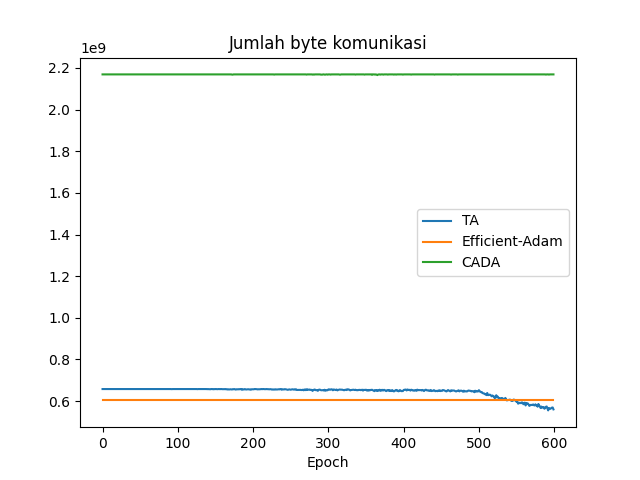
\includegraphics[width=0.8\columnwidth]{resources/resnet_bits.png}
  \caption{\label{resnetbits1}Communication data size used for each algorithm in CIFAR-10 scenario}
\end{figure}
\begin{figure}[htbp]
  \centering
  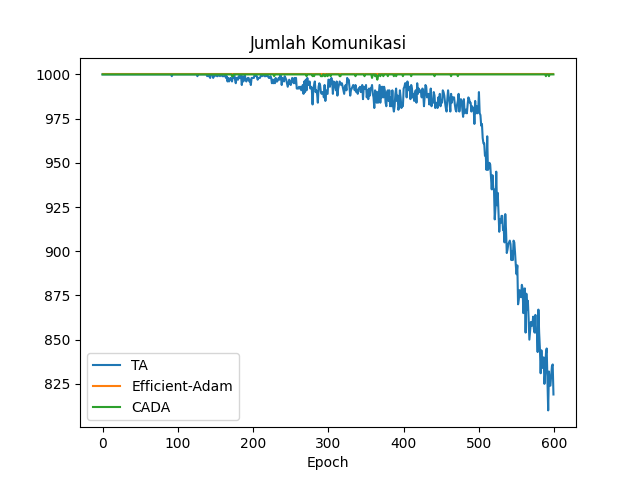
\includegraphics[width=0.8\columnwidth]{resources/resnet_comms.png}
  \caption{\label{resnetcomms1}Communication rounds for each algorithm in CIFAR-10 scenario}
\end{figure}

\subsection{Analysis}
From the two experiments, it could be seen that the more complex model has reduction in communication rounds, while the simpler model doesn't. The reduction in communication may be caused by the greater number of parameters ResNet-20 has, compared to the simpler model. The parameters will affect communication round because \autoref{cada2cond} dictates if a worker has gradient innovation smaller than the averaged parameter innovation over the last $d_\mathrm{max}$ iteration, the worker will skip sending updates. Therefore, reducing communication between worker and parameter server.
